\chapter{the representations of \texorpdfstring{$\mathfrak{sl}(3, \mathbb{C})$}{sl(3, C)}}
\begin{itemize}
	\item in this chapter, we are going to discuss the classification of the irreducible rep. of $\mathrm{SU}(3)$ and $\mathfrak{sl}(2, \mathbb{C})$.
	
	\item $\mathfrak{sl}(3, \mathbb{C}) \simeq \mathfrak{su}(3)_\mathbb{C}$.
	
	\item $\mathrm{SU}(m)$ are \textbf{simply connected}, \textbf{compact} Lie groups.
	\begin{itemize}
		\item according to subsection \ref{subsection 5.1.1}, 单连通李群 (的表示) 完全由其李代数 (的表示) 决定.
		
		rep. of $\mathfrak{sl}(3, \mathbb{C}) \overset{\text{restrict to}}{\Longrightarrow}$ rep. of $\mathfrak{su}(3) \overset{\text{simple connectedness}}{\Longrightarrow}$ rep. of $\mathrm{SU}(3)$.
		
		\item according to section \ref{5.2}, $\Pi$ is irreducible $\iff \pi$ is irreducible.
		
		and $\mathrm{SU}(3)$ is \textbf{compact}, so it has complete reducibility property $\Longrightarrow$ rep. of $\mathfrak{sl}(3, \mathbb{C})$ is \textbf{completely reducible}. 可见, 半单李代数的表示都是 completely reducible.
	\end{itemize}
\end{itemize}

\section{weights and roots}
\begin{itemize}
	\item 参考 subsection \ref{subsection 6.7.1}, 我们使用如下基矢,
	\begin{align}
		& H_1 = \begin{pmatrix}
			1 & & \\
			& - 1 & \\
			& & 0
		\end{pmatrix} \quad A_1 = \begin{pmatrix}
			0 & 1 & \\
			0 & 0 & \\
			& & 0
		\end{pmatrix} \quad B_1 = \begin{pmatrix}
			0 & 0 & \\
			1 & 0 & \\
			& & 0
		\end{pmatrix} \notag \\
		& H_2 = \begin{pmatrix}
			0 & & \\
			& 1 & \\
			& & - 1
		\end{pmatrix} \quad A_2 = \begin{pmatrix}
			0 & & \\
			& 0 & 1 \\
			& 0 & 0
		\end{pmatrix} \quad B_2 = \begin{pmatrix}
			0 & & \\
			& 0 & 0 \\
			& 1 & 0
		\end{pmatrix} \notag \\
		& A_3 = \begin{pmatrix}
			0 & & 1 \\
			& 0 & \\
			0 & & 0
		\end{pmatrix} \quad B_3 = \begin{pmatrix}
			0 & & 0 \\
			& 0 & \\
			1 & & 0
		\end{pmatrix} \label{12.1.1}
	\end{align}
	并注意到,
	\begin{equation}
		\mathrm{span}(H_1, A_1, B_1) \simeq \mathrm{span}(H_2, A_2, B_2) \simeq \mathrm{span}(H_1 + H_2, A_3, B_3) \simeq \mathfrak{sl}(2, \mathbb{C})
	\end{equation}
	
	\item 首先找到 roots,
	\begin{equation}
		\alpha_1 = H_1 \quad \alpha_2 = H_2 \quad \alpha_3 = H_1 + H_2 \quad \text{and} \quad \beta_i = - \alpha_i
	\end{equation}
	以及对应的 root vectors,
	\begin{equation}
		\mathfrak{g}_{\alpha_i} = \mathrm{span}(A_i) \quad \mathfrak{g}_{\beta_i} = \mathrm{span}(B_i)
	\end{equation}
	root system $A_2$ 如下,
	
	\begin{figure}[H]
		\centering
		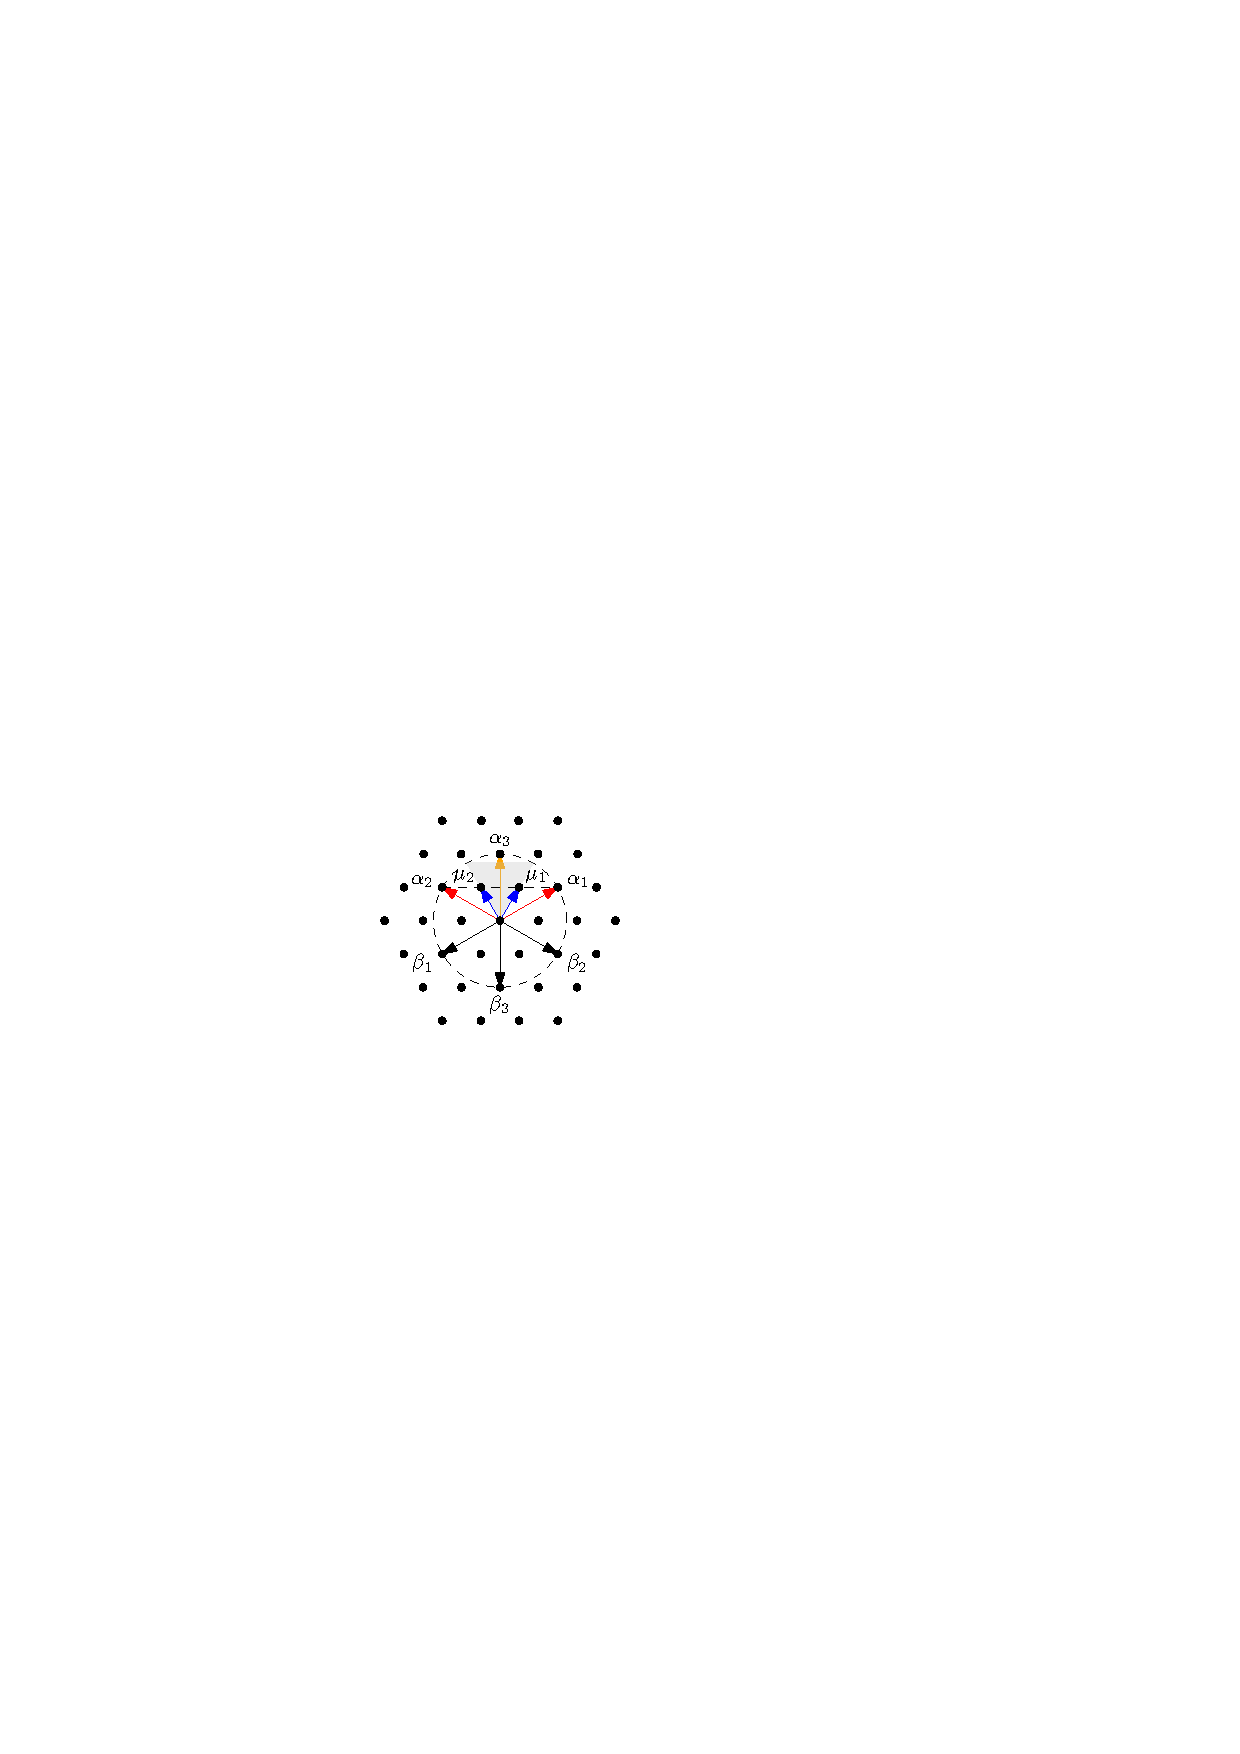
\includegraphics[scale=1]{figures/root system A2.pdf}
		\caption{root system $A_2$}
	\end{figure}
	
	\item 可见 $\alpha_1, \alpha_2$ 是 positive simple roots.
	
	\item 再来找 fundamental weights,
	\begin{equation}
		\mu_1 = \frac{2}{3} \alpha_1 + \frac{1}{3} \alpha_2 \quad \mu_2 = \frac{1}{3} \alpha_1 + \frac{2}{3} \alpha_2
	\end{equation}
\end{itemize}

\section{the irreducible representations}
\begin{itemize}
	\item 每个 dominant integral element (作为 highest weight) 对应一个 irreducible rep., 用 $(n_1, n_2)$ 代表 $n_1 \mu_1 + n_2 \mu_2$ 对应的 rep., 其中 $n_1, n_2 \in \mathbb{Z}_+ = \{0, 1, 2, \cdots\}$.
\end{itemize}

\subsection{the \texorpdfstring{$(1, 0)$}{(1, 0)} representation}
\begin{itemize}
	\item $(1, 0)$ rep. 中的 weights 有,
	\begin{equation}
		\mu_1 \quad \mu_1 - \alpha_1 \quad \mu_1 - \alpha_1 - \alpha_2
	\end{equation}
	
	\item $\mathfrak{h}$ 中的元素可以同时对角化为,
	\begin{equation}
		\pi_{(1, 0)}(H_1) = \begin{pmatrix}
			1 & & \\
			& - 1 & \\
			& & 0
		\end{pmatrix} \quad \pi_{(1, 0)}(H_2) = \begin{pmatrix}
			0 & & \\
			& 1 & \\
			& & - 1
		\end{pmatrix}
	\end{equation}
	其余元素的表示都是升降算符, 可见 $(1, 0)$ 表示就是 \eqref{12.1.1} 本身.
\end{itemize}

\subsection{the \texorpdfstring{$(0, 1)$}{(0, 1)} representation}
\begin{itemize}
	\item $(0, 1)$ rep. 中的 weights 有,
	\begin{equation}
		\mu_2 \quad \mu_2 - \alpha_2 \quad \mu_2 - \alpha_1 - \alpha_2
	\end{equation}
	
	\item $\mathfrak{h}$ 中的元素可以同时对角化为,
	\begin{equation}
		\pi_{(0, 1)}(H_1) = \begin{pmatrix}
			0 & & \\
			& 1 & \\
			& & - 1
		\end{pmatrix} \quad \pi_{(0, 1)}(H_2) = \begin{pmatrix}
			1 & & \\
			& - 1 & \\
			& & 0
		\end{pmatrix}
	\end{equation}
	其余元素的表示都是升降算符.
\end{itemize}

\subsection{the \texorpdfstring{$(1, 1)$}{(1, 1)} representation}
\begin{itemize}
	\item $(1, 1)$ rep. 中的 weights 有,
	\begin{align}
		& \mu_1 + \mu_2 \quad \mu_1 + \mu_2 - \alpha_1 \quad \mu_1 + \mu_2 - \alpha_2 \notag \\
		& \mu_1 + \mu_2 - \alpha_3 \quad \mu_1 + \mu_2 - \alpha_1 - \alpha_3 \quad \mu_1 + \mu_2 - \alpha_2 - \alpha_3 \quad \mu_1 + \mu_2 - 2 \alpha_3
	\end{align}
	
	\item 令,
	\begin{equation}
		v = \begin{pmatrix}
			1 \\
			0 \\
			0 \\
			0 \\
			0 \\
			0 \\
			0 \\
			0
		\end{pmatrix} \quad B_1 v = \begin{pmatrix}
			0 \\
			1 \\
			0 \\
			0 \\
			0 \\
			0 \\
			0 \\
			0
		\end{pmatrix} \quad B_2 v = \begin{pmatrix}
			0 \\
			0 \\
			1 \\
			0 \\
			0 \\
			0 \\
			0 \\
			0
		\end{pmatrix} \quad B_2 B_1 v = \begin{pmatrix}
			0 \\
			0 \\
			0 \\
			1 \\
			0 \\
			0 \\
			0 \\
			0
		\end{pmatrix} \quad B_1 B_2 v = \begin{pmatrix}
			0 \\
			0 \\
			0 \\
			0 \\
			1 \\
			0 \\
			0 \\
			0
		\end{pmatrix} \quad \cdots
	\end{equation}
	
	\item $\mathfrak{h}$ 中的元素可以同时对角化为,
	\begin{equation}
		H_1 = \begin{pmatrix}
			1 & & & & & & & \\
			& - 1 & & & & & & \\
			& & 2 & & & & & \\
			& & & 0 & & & & \\
			& & & & 0 & & & \\
			& & & & & - 2 & & \\
			& & & & & & 1 & \\
			& & & & & & & - 1
		\end{pmatrix} \quad H_2 = \begin{pmatrix}
			1 & & & & & & & \\
			& 2 & & & & & & \\
			& & - 1 & & & & & \\
			& & & 0 & & & & \\
			& & & & 0 & & & \\
			& & & & & 1 & & \\
			& & & & & & - 2 & \\
			& & & & & & & - 1
		\end{pmatrix}
	\end{equation}
	其它元素的表示都是升降算符,
	\begin{align}
		& \pi_{(1, 1)}(A_1) = \begin{pmatrix}
			0 & 1 & & & & & & \\
			& 0 & & & & & & \\
			& & 0 & 1 & 2 & & & \\
			& & & 0 & & & & \\
			& & & & 0 & - 1 & & \\
			& & & & & 0 & & \\
			& & & & & & 0 & - 2 \\
			& & & & & & & 0
		\end{pmatrix} \quad \pi_{(1, 1)}(B_1) = \pi_{(1, 1)}(A_1)^T \notag \\
		& \pi_{(1, 1)}(A_2) = \begin{pmatrix}
			0 & & 1 & & & & & \\
			& 0 & & 2 & 1 & & & \\
			& & 0 & & & & & \\
			& & & 0 & & & 1 & \\
			& & & & 0 & & & \\
			& & & & & 0 & & 2 \\
			& & & & & & 0 & \\
			& & & & & & & 0
		\end{pmatrix} \quad \pi_{(1, 1)}(B_2) = \pi_{(1, 1)}(A_2)^T \notag \\
		& \pi_{(1, 1)}(A_3) = \begin{pmatrix}
			0 & & & 1 & - 1 & & & \\
			& 0 & & & & 1 & & \\
			& & 0 & & & & 1 & \\
			& & & 0 & & & & 2 \\
			& & & & 0 & & & - 2 \\
			& & & & & 0 & & \\
			& & & & & & 0 & \\
			& & & & & & & 0
		\end{pmatrix} \quad \pi_{(1, 1)}(B_3) = \pi_{(1, 1)}(A_3)^T
	\end{align}
	可以验证这确实是 $\mathfrak{sl}(3, \mathbb{C})$ 的一个表示.
\end{itemize}

\section{strong interaction and \texorpdfstring{$\mathfrak{sl}(3, \mathbb{C})$}{sl(3, C)}}
\begin{itemize}
	\item 
\end{itemize}
